\documentclass[11]{article}

\usepackage{graphicx}
\usepackage{hyperref}
\usepackage{subcaption}
\usepackage{amsmath}
\usepackage[
    backend=bibtex,
%    isbn=false,
%    url=false,
%    doi=false,
%    eprint=false,
%    hyperref=false,
%    backref=false,
%    firstinits=false,
]{biblatex}
\bibliography{references}

\hypersetup{colorlinks,urlcolor=blue}
\let \shorttitle \textbf
\begin{document}

\section{Introduction}
Tool use is one of the human abilities that uniquely distinguishes man from other species. 
We refer to tools as hand held devices used in making changes to the surrounding environment. 
Cases of tool use have been reported in other species, but never to the magnitude engaged by humans \cite{boysen1999,harrington2009,lefebvre2004}. 
As a defining attribute of human cognition, we wish to lay the foundations for a computational model of the reasoning processes involved.

\subsection{The four constraints theory}
Our model stems from the architectural framework defined by the four constraints theory (4CT) \cite{osiurak2014a}.
4CT characterises tool use for healthy individual's behaviour.
Its theoretical basis lie however on the empirical investigations of aprxia and the cognitive impairments caused.
Apraxia is a neurological disorder impairing a person's ability to plan and execute sequences of movements.
The term covers a multitude of symptoms and levels of severity (e.g. dyspraxia, ideomotor aparaxia, apraxia of speech) .
The underlying cause for these disorders is physical damage to the left hemisphere of the brain\cite{osiurak2013}.

\begin{figure}[h]
  \centering
  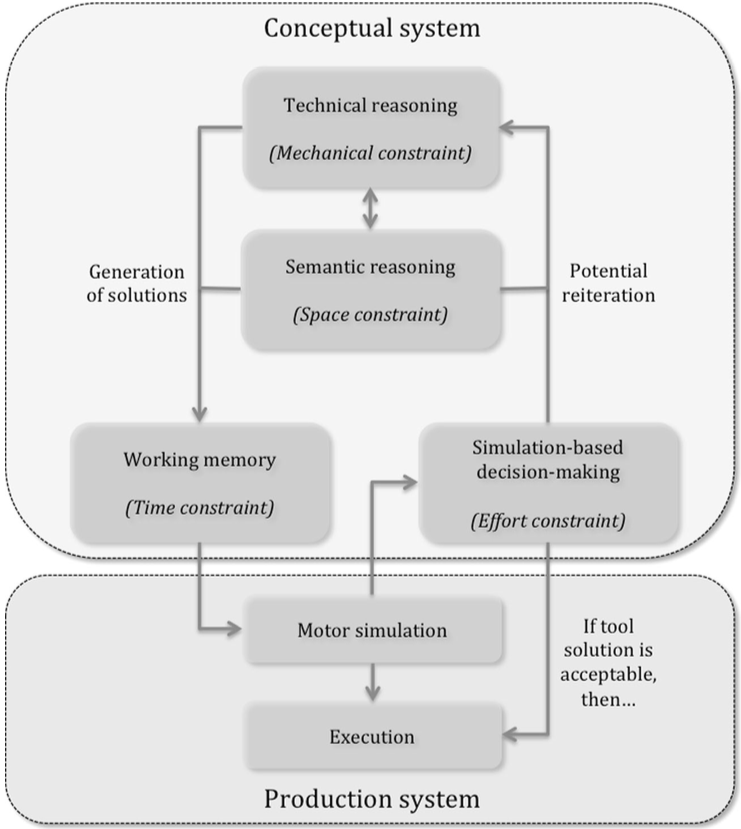
\includegraphics[width=.9\textwidth]{./figures/4CTArchitecture.png}
  \caption{4CT architecture reprinted from \cite{osiurak2014a}}
  \label{fig:4CTArchitecture}
\end{figure}      

4CT structures tool use into a conceptual system and a production system (fig. \ref{fig:4CTArchitecture}).
The theory mostly focuses on the conceptual level which encapsulates cognitive reasoning.
Task execution is handled by the production system which dictates motor movement.   
Due to the distinction, 4CT's conceptual system is a suitable candidate for a computational model concentrated on reasoning.

%-----------
% More paragraphs needed to explain why 4CT is desired over other theories
%-----------

The theory outlines tool use situations as problem solving tasks. 
Even the simple scenario of slicing bread requires reasoning about the knife's sharpness,length, hardness, and the movements necessary to manifest mechanical effects like cutting. 
Problem solving becomes even more apparent in the absence of familiar tools, when subjects are required to fashion their own. 

The four constraints of \emph{mechanics, space, time,} and \emph{effort} are the dimensions within which problem solving tasks are defined.
Aiding problem solving are four corresponding processes: \emph{technical reasoning, semantic reasoning, working memory,} and \emph{simulation based decision making} (fig. \ref{fig:4CTArchitecture}).  


\printbibliography
\end{document}
